\documentclass{article}
\setlength{\oddsidemargin}{0.25 in}
\setlength{\evensidemargin}{-0.25 in}
\setlength{\topmargin}{-0.6 in}
\setlength{\textwidth}{6.5 in}
\setlength{\textheight}{8.5 in}
\setlength{\headsep}{0.75 in}
\setlength{\parindent}{0 in}
\setlength{\parskip}{0.1 in}
\usepackage{amssymb}
\usepackage{amsmath,amsfonts,graphicx}
\usepackage{hyperref}
\usepackage{enumitem}

\newcounter{lecnum}

\renewcommand{\thepage}{\thelecnum-\arabic{page}}
\renewcommand{\thesection}{\thelecnum.\arabic{section}}
\renewcommand{\theequation}{\thelecnum.\arabic{equation}}
\renewcommand{\thefigure}{\thelecnum.\arabic{figure}}
\renewcommand{\thetable}{\thelecnum.\arabic{table}}

%
% The following macro is used to generate the header.
%
\newcommand{\lecture}[4]{
   \pagestyle{myheadings}
   \thispagestyle{plain}
   \newpage
   \setcounter{lecnum}{#1}
   \setcounter{page}{1}
   \noindent
   \begin{center}
   \framebox{
      \vbox{\vspace{2mm}
    \hbox to 6.28in { {\bf CS 768: Learning With Graphs
        \hfill Autumn 2020-2021} }
       \vspace{4mm}
       \hbox to 6.28in { {\Large \hfill Lecture #1: #2  \hfill} }
       \vspace{2mm}
       \hbox to 6.28in { {\it Instructor: Prof. Abir De \hfill Scribe: #4} }
      \vspace{2mm}}
   }
   \end{center}
   \markboth{Lecture #1: #2}{Lecture #1: #2}
}

%Use this command for a figure; it puts a figure in wherever you want it.
%usage: \fig{NUMBER}{SPACE-IN-INCHES}{CAPTION}
\newcommand{\fig}[3]{
            \vspace{#2}
            \begin{center}
            Figure \thelecnum.#1:~#3
            \end{center}
    }
% Use these for theorems, lemmas, proofs, etc.
\newtheorem{theorem}{Theorem}[lecnum]
\newtheorem{lemma}[theorem]{Lemma}
\newtheorem{proposition}[theorem]{Proposition}
\newtheorem{claim}[theorem]{Claim}
\newtheorem{corollary}[theorem]{Corollary}
\newtheorem{definition}[theorem]{Definition}
\newenvironment{proof}{{\bf Proof:}}{\hfill\rule{2mm}{2mm}}

% **** IF YOU WANT TO DEFINE ADDITIONAL MACROS FOR YOURSELF, PUT THEM HERE:
\newcommand{\Sim}{\text{sim}}

\begin{document}

\lecture{10}{Supervised Random Walk}{}{Arjit Jain \& Samad Koita}

\section{Supervised Link Prediction Methods}
\begin{enumerate}
\item Combining scores of different unsupervised methods
\begin{itemize}
    \item Computing Scores: $s_w(u,v) = w_{AA}AA(u,v) + w_{CN}CN(u,v) + b$
    \item Learning Weights: SVM/Ranking loss on scores
\end{itemize}
\item Supervised Random Walk
\item Collaborative Filtering based approaches
\end{enumerate}
\section{Precursor: Random Walks on Graphs}
\subsection{Link Prediction with Random Walks} 

Consider a source node $s \in V$ in the Graph $ G = (V,E)$. Let $D = (d_1, d_2, \ldots ,d_n)$ be the candidate neighbours (or destination nodes) of node $s$. We assume that $s$ and $d$ are likely to be connected in the future if:
\begin{itemize}
    \item The structure around $s$ and $d$ is rich - their surrounding region has a lot of edges.
    \item There is some affinity between $s$ and $d$
\end{itemize}
One way to judge how rich the structure is around $s$ and $d$ is using random walks. Let $count(s,d)$ is the number of times $d$ is reached in a random walk starting at $s$. Let $p(s,d)$ be the probability of reaching $d$ from a random walk starting at s. We define $score(s,d)$ as:$$
score(s,d) \propto count(s,d) \propto p(s,d)$$
Once we obtain the scores for each $d_i \in D$, we can evaluate this approach for link prediction using MAP or Average Precision.
\begin{figure}[!htb]
\minipage{0.5\textwidth}
  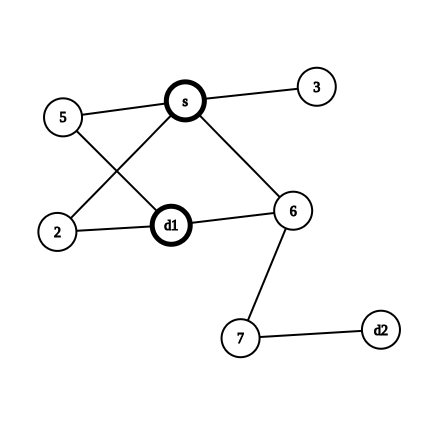
\includegraphics[width=\linewidth]{graph_random_walk_d2.png}
  \caption{Edge ($s$,$d_1$) -  High probability}\label{fig:awesome_image1}
\endminipage\hfill
\minipage{0.5\textwidth}
  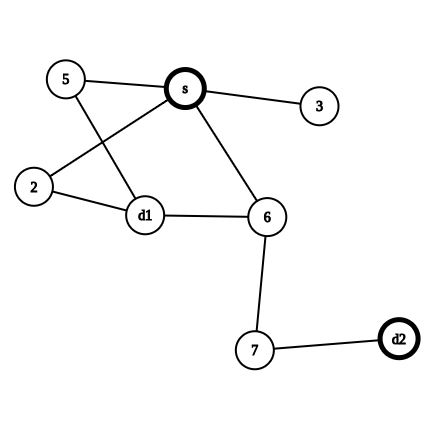
\includegraphics[width=\linewidth]{graph_random_walk_d1.png}
  \caption{Edge ($s$,$d_2$) -  Low probability}\label{fig:awesome_image2}
\endminipage\hfill
\end{figure}
\subsection{Constructing a Random Walk} 
Consider the graph  $ G = (V,E)$. Let $A$ be the adjacency matrix of the graph. $A_{ij} = 1$ if vertex $v_i$ is connected to $v_j$, and $0$ otherwise. How to perform a random walk on this graph?
To do this we define the transition matrix $\mathbf P$.\\
\textbf{Transition Matrix:} $\mathbf P$ is said to be the transition matrix of a graph when $\forall i,j \; P_{ij}$ denotes the probability that $v_i$ follows $v_j$ in a random walk on the graph. Since you can only move to neighbouring nodes, $(A_{ij} =0) \implies (P_{ij} = 0)$. $P$ is a stochastic matrix - the sum of entries in each row is 1.
\\
Once we have this matrix $\mathbf P$, we can use it to computer the probability of reaching one node from the other. Using these probabilities, we can compute $score(s,d)$.
\\
Traditional Random Walks assume you are equally likely to visit each one of your neighbours, and choose $P$ in such a way that this condition is satisfied. \\Supervised Random Walks get around this assumption. Using both node features, and the structure of the graph, the transition matrix $P$ is learnt. 

\subsection{Computing Scores: PageRank}
Given a transition matrix, also called weighted adjacency matrix, $\mathbf P$, and nodes $s$ and $d$, how to compute $score(s,d)$?
Let us analyse $\mathbf P$ a little closely. Let $P(j|i) = P_{ij}$ be the probability of the moving to node j from the node i in a random walk.
\begin{equation*}
    P_ i = 
    \begin{bmatrix}
    P(1 | i) & P(2 | i) & \dots & P(n | i) 
    \end{bmatrix}
\end{equation*}
$\mathbf P$ is a stochastic matrix, having sum of each row as 1. Therefore,
\begin{equation*}
    \mathbf{P^M}
    \begin{bmatrix}
    1 \\ 1 \\ \vdots \\ 1
    \end{bmatrix} = 
    \mathbf{P}
    \begin{bmatrix}
    1 \\ 1 \\ \vdots \\ 1
    \end{bmatrix} = 
    \begin{bmatrix}
    1 \\ 1 \\ \vdots \\ 1
    \end{bmatrix}
\end{equation*}
From the equation above, we can see that $\lambda(\mathbf{P}) = 1$.\\
Given a starting state $s$, let $p_t = \begin{bmatrix}
    p_{1t} & \dots & p_{nt} 
    \end{bmatrix}$ where $p_{it}$ is the probability of being at node $i$ after t steps.
\begin{equation*}
    p_t^T \mathbf{P} \; = \; p_{t+1}^T
\end{equation*}
\textbf{Stationary Distribution:} As $t\to \infty$, the probability of being at any node $p_{\infty}^T$ will be:
\begin{equation*}
    p_{\infty}^T \; = \; \lim_{t \to \infty}{(p_0^T \mathbf{P}^t)}
\end{equation*}
In most cases, this limit exists, and $p_{\infty} = p_{st}$, the steady state probability distribution on the graph. Clearly, $    p_{\infty}^T \; = \; p_{st}^T \mathbf{P}$. This implies $p_{st}$ is the left eigenvector of the eigenvalue $\lambda = 1$ of $\mathbf{P}$.\par
This steady state distribution, $p_{st}$ is called the {\it PageRank} of the graph.
\par
We have defined $score(s,d)$ to be proportional to the probability of reaching a node $d$ in a random walk. Hence we define:
$$score(s,d) = p_{st}[d]$$

\subsection{Better Metric: Personalised PageRank}
An interesting ovservation is that $score(s,d) = p_{st}[d]$ is independent of the start node $s$. Therefore, for the purpose of link prediction, simply using PageRank is not enough to make user-specific predictions. We correct for this by introducing personalised page rank.\\
The idea is to introduce a restart probability, with which, a node can jump back to the source vertex $s$. This biases the random walks to the starting node $s$, and hence more localized, or personalized, compared to PageRank.  
\begin{equation*}
    P^*_{ij} = (1-\alpha)P_{ij} + \alpha I(j=s)
\end{equation*}
where $\alpha$ is the restart probability.\\
Hence, 
\begin{equation*}
    P^*_{s} = (1-\alpha)P + \alpha R_s
\end{equation*}
where only the entries in $s^{th}$ column of $R_s$ are $1$, and all others are $0$. 
\\Note that
\begin{equation*}
    \mathbf{P^*}
    \begin{bmatrix}
    1 \\ 1 \\ \vdots \\ 1
    \end{bmatrix} = 
    (1-\alpha)\mathbf{P}
    \begin{bmatrix}
    1 \\ 1 \\ \vdots \\ 1
    \end{bmatrix} + \alpha R_s \begin{bmatrix}
    1 \\ 1 \\ \vdots \\ 1
    \end{bmatrix} 
    \\= 
    (1-\alpha)
    \begin{bmatrix}
    1 \\ 1 \\ \vdots \\ 1
    \end{bmatrix} + \alpha \begin{bmatrix}
    1 \\ 1 \\ \vdots \\ 1
    \end{bmatrix} 
    = 
    \begin{bmatrix}
    1 \\ 1 \\ \vdots \\ 1
    \end{bmatrix}
\end{equation*}
Similar to the above derivation, we can derive $p^T_s$ to be the solution of 
\begin{equation*}
    p^T \mathbf{P^*_s} \; = \; p^T
\end{equation*}
\section{Supervised Random Walk}
\subsection{Modelling the Transition Matrix}
One way to model the transition matrix $P$ with the parameter $w$ is as follows:
\begin{equation*}
    P_{ij} = \frac{w^Tf(x_i, x_j)}{\sum_{j'}{w^Tf(x_i, x_{j'})}}
\end{equation*}
where $x_i, x_j$ are the node features of nodes $i$ and $j$ respectively.\\
Here, $f$ should be a non-negative function, for example\\
$f(x, y) = ||x-y||$ (Norm function)\\
$f(x, y) = x \odot y$ (Element-wise dot product)\\
The requirement of a non negative function can be bypassed using a hinge as follows:
\begin{equation*}
    P_{ij} = \frac{[w^Tf(x_i, x_j)]_+}{\sum_{j'}{[w^Tf(x_i, x_{j'})]_+}}
\end{equation*}
Incorporating constraints:\\
For a fixed node $s$, we choose $w$ as per the following objective
$$\min ||w||^2 $$ such that $\forall l, d\ (s, l) \notin E, (s, d) \in E\ \ \  p^T_s[d] = P_\infty (d|s) > P_\infty (l|s) = p^T_s[l]$
\\
i.e. the min norm solution of $w$ such that the probabilities, as computed by Personalized PageRank using parameter $w$, for neighbours of $s$ are more than  non-neighbours.\\
Hence, for a node $s$, we have $N(s) \times (|V| - N(s))$ constraints.\\
\\
Note that, the optimal $w$ can be calculated either individually for all source nodes $s$, or a common $w$ can be calculated across all nodes. \\
In practice, the above optimization can be realised using hinge loss and some form of regularization on $w$.
i.e. 
$$\min\  \lambda ||w||^2 + \sum_{l, d\ (s, l) \notin E, (s, d) \in E}{[p^T_s[l]-p^T_s[d]]_+}$$
\subsection{Recommended reading}
\href{https://cs.stanford.edu/~jure/pubs/linkpred-wsdm11.pdf}{Supervised Random Walks: Predicting and Recommending Links in Social Networks}\cite{wsdm}
\bibliographystyle{acm}
\bibliography{ref}
\end{document}